\documentclass[12pt]{article}
\usepackage[margin=1in]{geometry}
\usepackage{setspace}
\onehalfspacing

% Start of preamble
%==========================================================================================%
% Required to support mathematical unicode
\usepackage[warnunknown, fasterrors, mathletters]{ucs}
\usepackage[utf8x]{inputenc}

\usepackage[dvipsnames,table,xcdraw]{xcolor}

% Standard mathematical typesetting packages
\usepackage{amsmath,amssymb,amscd,amsthm,amsxtra, pxfonts}
\usepackage{mathtools,mathrsfs,dsfont,xparse}

% Symbol and utility packages
\usepackage{cancel, textcomp}
\usepackage[mathscr]{euscript}
\usepackage[nointegrals]{wasysym}
\usepackage{apacite}

% Extras
\usepackage{physics}  
\usepackage{tikz-cd} 
\usepackage{microtype}
\usepackage{enumitem}
\usepackage{titling}
\usepackage{graphicx}

% Fancy theorems due to @intuitively on discord
\usepackage{mdframed}
\newmdtheoremenv[
backgroundcolor=NavyBlue!30,
linewidth=2pt,
linecolor=NavyBlue,
topline=false,
bottomline=false,
rightline=false,
innertopmargin=10pt,
innerbottommargin=10pt,
innerrightmargin=10pt,
innerleftmargin=10pt,
skipabove=\baselineskip,
skipbelow=\baselineskip
]{mytheorem}{Theorem}

\newenvironment{theorem}{\begin{mytheorem}}{\end{mytheorem}}

\newtheorem{corollary}{Corollary}
\newtheorem{lemma}{Lemma}

\newtheoremstyle{definitionstyle}
{\topsep}%
{\topsep}%
{}%
{}%
{\bfseries}%
{.}%
{.5em}%
{}%
\theoremstyle{definitionstyle}
\newmdtheoremenv[
backgroundcolor=Violet!30,
linewidth=2pt,
linecolor=Violet,
topline=false,
bottomline=false,
rightline=false,
innertopmargin=10pt,
innerbottommargin=10pt,
innerrightmargin=10pt,
innerleftmargin=10pt,
skipabove=\baselineskip,
skipbelow=\baselineskip,
]{mydef}{Definition}
\newenvironment{definition}{\begin{mydef}}{\end{mydef}}

\newtheorem*{remark}{Remark}

\newtheorem*{example}{Example}

% Common shortcuts
\def\mbb#1{\mathbb{#1}}
\def\mfk#1{\mathfrak{#1}}

\def\bN{\mbb{N}}
\def \C{\mbb{C}}
\def \R{\mbb{R}}
\def\bQ{\mbb{Q}}
\def\bZ{\mbb{Z}}
\def \cph{\varphi}
\renewcommand{\th}{\theta}
\def \ve{\varepsilon}
\newcommand{\mg}[1]{\| #1 \|}

% Often helpful macros
\newcommand{\floor}[1]{\left\lfloor#1\right\rfloor}
\newcommand{\ceil}[1]{\left\lceil#1\right\rceil}
\renewcommand{\qed}{\hfill\qedsymbol}
\renewcommand{\P}{\mathbb P\qty}
\newcommand{\E}{\mathbb{E}\qty}
\newcommand{\Cov}{\mathrm{Cov}\qty}
\newcommand{\Var}{\mathrm{Var}\qty}

% Sets
\usepackage{braket}

\graphicspath{{/}}
\usepackage{float}

\newcommand{\SET}[1]{\Set{\mskip-\medmuskip #1 \mskip-\medmuskip}}

% End of preamble
%==========================================================================================%

% Start of commands specific to this file
%==========================================================================================%

\usepackage{listings}
\lstset{
  columns=flexible,
  basicstyle=\small\ttfamily,
  mathescape=true,
  escapeinside=||
}
\usepackage{subcaption}

%==========================================================================================%
% End of commands specific to this file

\title{CSE Template}
\date{\today}
\author{Rohan Mukherjee}

\begin{document}
    \maketitle
    \subsection*{1.1.3}
    \begin{enumerate}
        \item I think the main reason cosine similarity works better than other distance metrics like L1/L2 is because it is norm-invariant. If you have two sentence embeddings $x$ and $y$, and these were really similar, one would expect that $2x$ and $2y$ would be really similar too. In fact, you would think these would be just as similar as $x$ and $y$. This is only true for cosine similarity. 
        \item It chooses option a, pessimistic, instead. Recall that the Glove representation we are using for words is the context based wordvec model. Although positive and sanguine are synonyms, it is more likely that pessimistic has a context more simliar to sanguine than to pessimistic. Of course these words are similar, being antonyms, and there is no way to tell the difference between synonyms and antonyms with Glove. 
        \item I created the following questions:

        \textbf{Question 1:} Relation: Synonyms \\
        Car is to automobile as bike is to \underline{\hspace{2cm}}?

        \begin{enumerate}
            \item[a)] horse
            \item[b)] \fbox{bicycle}
            \item[c)] house
            \item[d)] oranges
        \end{enumerate}

        \textbf{Question 2:} Relation: Synonyms \\
        House is to residence as cow is to \underline{\hspace{2cm}}?

        \begin{enumerate}
            \item[a)] bus
            \item[b)] horse
            \item[c)] air
            \item[d)] \fbox{bull}
        \end{enumerate}

        \textbf{Question 3:} Relation: Antonyms \\
        Happy is to sad as good is to \underline{\hspace{2cm}}?

        \begin{enumerate}
            \item[a)] \fbox{bad}
            \item[b)] horse
            \item[c)] water
            \item[d)] cow
        \end{enumerate}

        \textbf{Question 4:} Relation: Antonyms \\
        Big is to small as fast is to \underline{\hspace{2cm}}?

        \begin{enumerate}
            \item[a)] \fbox{slow}
            \item[b)] horse
            \item[c)] water
            \item[d)] feline
        \end{enumerate}

        \textbf{Question 5:} Relation: Taxonomy (Basic/Subordinate) \\
        Car is to vehicle as apple is to \underline{\hspace{2cm}}?

        \begin{enumerate}
            \item[a)] \fbox{fruit}
            \item[b)] horse
            \item[c)] water
            \item[d)] air
        \end{enumerate}

        \textbf{Question 6:} Relation: Taxonomy (Basic/Subordinate) \\
        Horse is to animal as chair is to \underline{\hspace{2cm}}?

        \begin{enumerate}
            \item[a)] fruit
            \item[b)] \fbox{furniture}
            \item[c)] water
            \item[d)] air
        \end{enumerate}

        \item First, here is the graph of the effect sizes vs vector sizes with the number of tokens fixed at 6B:
        \begin{figure}[H]
            \centering
            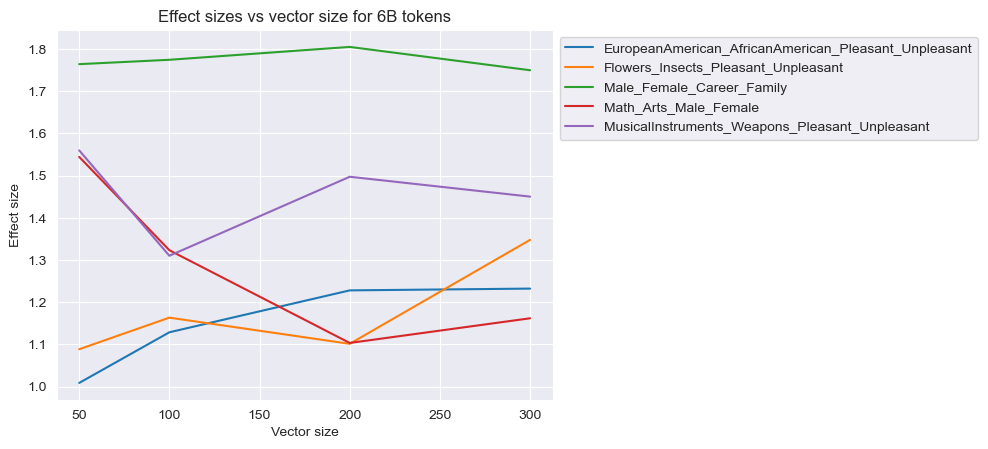
\includegraphics[width=0.8\textwidth]{images/effect_sizes_6b_tokens.png}
            \caption{Effect size vs Vector size}
        \end{figure}
        Here is the graph of the effect sizese vs number of tokens with vector size fixed at 300:
        \begin{figure}[H]
            \centering
            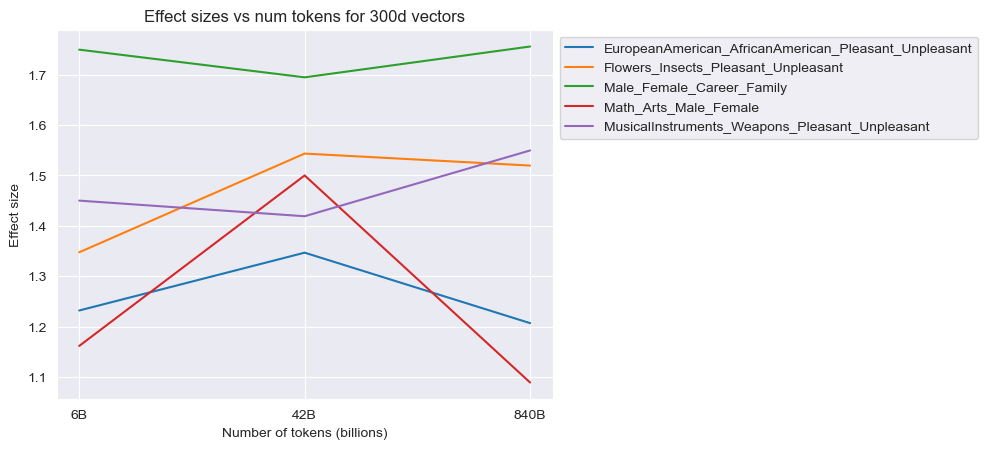
\includegraphics[width=0.8\textwidth]{images/effect_sizes_300d_vectors.png}
            \caption{Effect size vs Number of tokens}
        \end{figure}
        For both vector sizes and the number of tokens, the male female career family is held basically constant, same with musical instruments weapons. For math arts male female, the effect size drops as both the number of tokens and vector size increase. However, weirdly enough the middle token size of 42B it goes sharply up, then back sharply down. For the other two, they seem to increase at a slow rate. 
    \end{enumerate}

    \subsection*{1.2.2}
    \begin{enumerate}
        \item The main problem is not understanding the context of our words. This model does not have any sense of the position of the words, so we could do "This movie is great and everyone who says otherwise is totally wrong, and abhorrent!". With no understanding of context this will fail drastically. Similarly, someone could say something like "This movie is great, but the second actor was bad". It is likely this would have a similar sum to "This movie is bad, but the second actor is great". 
        \item Here is the graph of k vs accuracies:
        \begin{figure}[H]
            \centering
            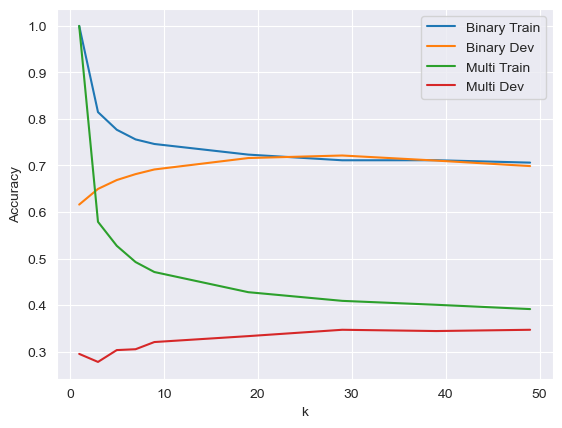
\includegraphics[width=0.8\textwidth]{images/effect_of_k_on_knn.png}
            \caption{k vs Accuracy}
        \end{figure}
        I notice that training accuracy moves consistently down, but the dev accuracy seems to increase up to a point. This is clear, as with k = 1 the model will just predict the same label because it has memorized the training data, and will do very bad on the dev data, as it hasn't. When k increases you get more generalizability, so the dev accuracy increases. But after a while, it gets gradually worse, as taking k to be the entire training set would always just output the same label. You would start comparing it to things that are not relevant. 
    \end{enumerate}

    \subsection*{2.2}
    \begin{enumerate}
        \item Say we set a max number of words of 2048. Then if we used padding instead of a sentence transformer, for the overwhemling majority of sentences, most of the words word be padding. This would mean that the overwhelming majority of our parameters would be useless most of the time, and the few times they are used they haven't been trained enough. So you would see a huge case of overfitting and poor generalizability. 

        \item Some of the issues I raised above happen when using the Glove representations vs sentence transformers. One notable example is: "And if you're not nearly moved to tears by a couple of scenes, you've got ice water in your veins." This follows almost the exact framework I said above: "This movie is (postiive word) and if you disagree you are (negative word)". Of course the Glove reps would be confused because this is the same sentence as "This movie is (negative word) and if you disagree you are (positive word)". The sentence transformers would be able to understand the context of the words and would be able to differentiate between the two. THe seame logic applies to "The film serves as a valuable time capsule to remind us of the devastating horror suffered by an entire people ." 

        \newpage
        \item Here is a comparison of binary and multi models with different configurations of units and layers for loss and accuracy.

        \begin{figure}[h!]
            \centering
        
            % First Row
            \begin{subfigure}{0.35\textwidth}
                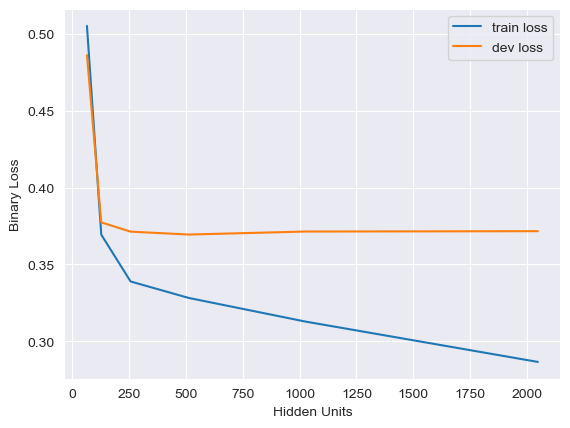
\includegraphics[width=\textwidth]{images/binary_units_loss.png}
                \caption{Binary - Units - Loss}
            \end{subfigure}
            \hfill
            \begin{subfigure}{0.35\textwidth}
                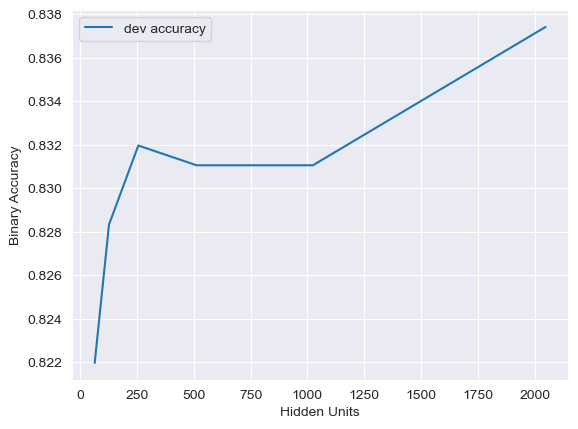
\includegraphics[width=\textwidth]{images/binary_units_acc.png}
                \caption{Binary - Units - Accuracy}
            \end{subfigure}
        
            % Second Row
            \begin{subfigure}{0.35\textwidth}
                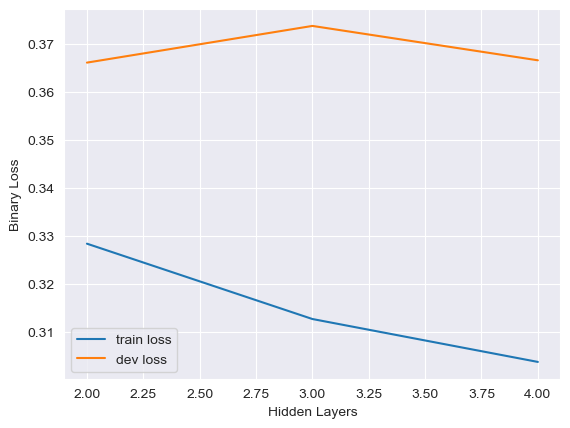
\includegraphics[width=\textwidth]{images/binary_layers_loss.png}
                \caption{Binary - Layers - Loss}
            \end{subfigure}
            \hfill
            \begin{subfigure}{0.35\textwidth}
                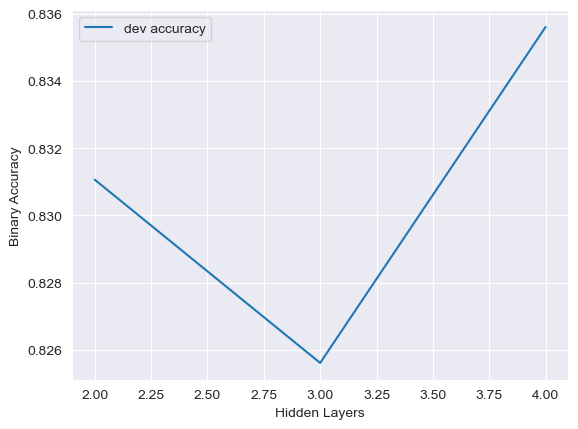
\includegraphics[width=\textwidth]{images/binary_layers_acc.png}
                \caption{Binary - Layers - Accuracy}
            \end{subfigure}
        
            % Third Row
            \begin{subfigure}{0.35\textwidth}
                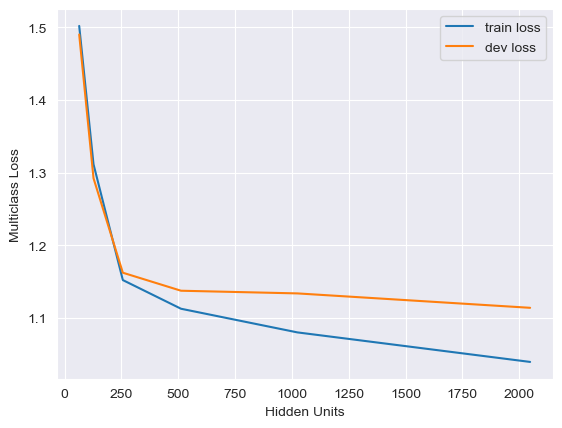
\includegraphics[width=\textwidth]{images/multi_units_loss.png}
                \caption{Multi - Units - Loss}
            \end{subfigure}
            \hfill
            \begin{subfigure}{0.35\textwidth}
                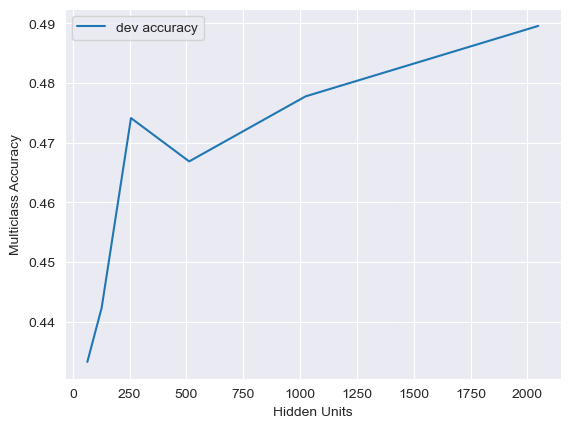
\includegraphics[width=\textwidth]{images/multi_units_acc.png}
                \caption{Multi - Units - Accuracy}
            \end{subfigure}
        
            % Fourth Row
            \begin{subfigure}{0.35\textwidth}
                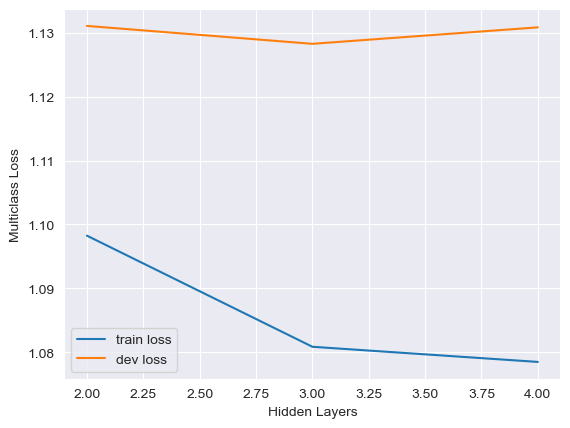
\includegraphics[width=\textwidth]{images/multi_layers_loss.png}
                \caption{Multi - Layers - Loss}
            \end{subfigure}
            \hfill
            \begin{subfigure}{0.35\textwidth}
                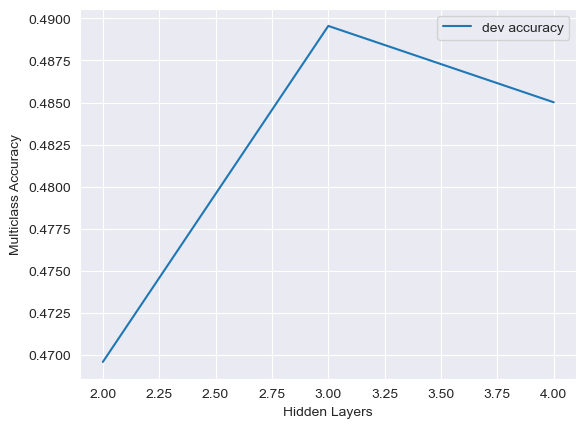
\includegraphics[width=\textwidth]{images/multi_layers_acc.png}
                \caption{Multi - Layers - Accuracy}
            \end{subfigure}
            \label{fig:graphs}
        \end{figure}

        We observe on both parts that generally, having more units up to a point decreases dev loss and increases accuracy. With the hidden units too low, the linear layers are just not complex enough to understand the problem at hand. However, the model depth seems to just not work very well (in the binary case, the loss is confusing and the accuracy gains are very small on the order of 1\%). Using the default parameters, I believe this is probably related to the fact that the number of epochs is too small, or maybe the learning rate too large (since the gradients could start to grow very large as the number of layers increase). When I tried increasing the number of epochs, I realized that it was actually overfitting with 4 layers. This is pretty surprising to me! Most of the time 1 hidden layer got the best results. 

        Here is the graph for SIQA:
        \begin{figure}[h!]
            \centering
        
            % Top Row (Units)
            \begin{subfigure}{0.45\textwidth}
                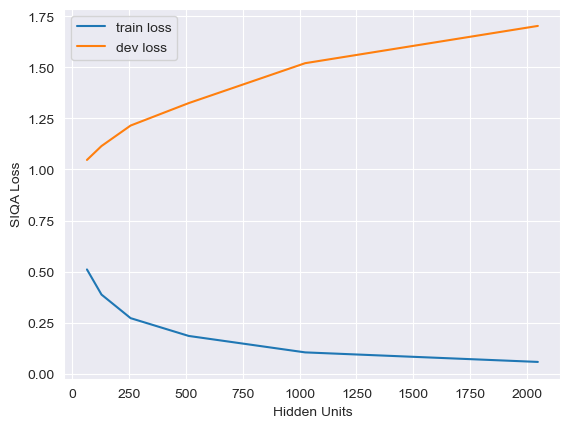
\includegraphics[width=\textwidth]{images/siqa_units_loss.png}
                \caption{SIQA - Units - Loss}
            \end{subfigure}
            \hfill
            \begin{subfigure}{0.45\textwidth}
                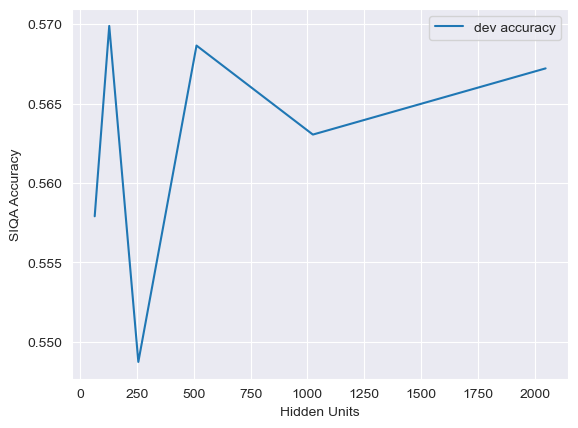
\includegraphics[width=\textwidth]{images/siqa_units_acc.png}
                \caption{SIQA - Units - Accuracy}
            \end{subfigure}
        
            % Bottom Row (Layers)
            \begin{subfigure}{0.45\textwidth}
                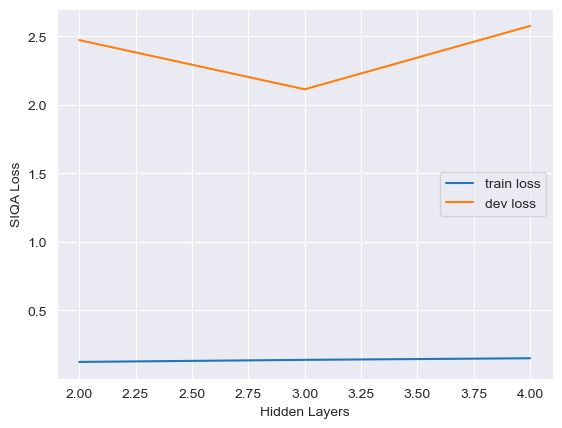
\includegraphics[width=\textwidth]{images/siqa_layers_loss.png}
                \caption{SIQA - Layers - Loss}
            \end{subfigure}
            \hfill
            \begin{subfigure}{0.45\textwidth}
                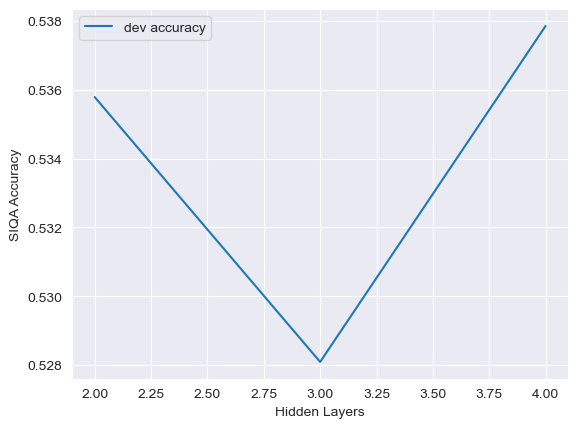
\includegraphics[width=\textwidth]{images/siqa_layers_acc.png}
                \caption{SIQA - Layers - Accuracy}
            \end{subfigure}
        
            \caption{SIQA results comparing units and layers configurations for loss and accuracy.}
            \label{fig:siqa_results}
        \end{figure}
        Here we see a catastrophic case of overfitting for both models. The loss dips lower and lower for the training data, yet the dev loss and accuracy are all over the place. The same happens with the number of layers, but surprisingly, the training loss stays at about the same place. When I trained on 40 epochs, the training loss dipped to 0.06, while the dev loss skyrocketed to 2.9. This is clear case of overfitting.

    \end{enumerate}
\end{document}